% One-page stakeholder summary: CSR agent architecture (DAG) + reliability-as-education framing.
% Build: cd docs && pdflatex csr_dag_agent_onepager.tex
\documentclass[10pt]{article}
\usepackage[letterpaper,margin=0.6in,top=0.5in,bottom=0.5in]{geometry}
\usepackage[T1]{fontenc}
\renewcommand{\ttdefault}{pcr}
\usepackage[scaled]{helvet}
\renewcommand{\familydefault}{\sfdefault}
\usepackage{xcolor}
\usepackage{tikz}
\usetikzlibrary{arrows.meta,positioning,calc}
\usepackage{enumitem}
\usepackage{booktabs}
\usepackage{tabularx}
\usepackage{titlesec}
\usepackage[hidelinks]{hyperref}

\definecolor{navy}{HTML}{1F3A5F}
\definecolor{accent}{HTML}{2E86AB}
\definecolor{soft}{HTML}{EAF2F8}
\definecolor{warn}{HTML}{C0392B}
\definecolor{ok}{HTML}{1E8449}
\definecolor{muted}{HTML}{5D6D7E}

\pagestyle{empty}
\setlength{\parindent}{0pt}
\setlength{\parskip}{3pt}
\titleformat{\section}{\color{navy}\bfseries\large}{}{0pt}{}[{\color{accent}\titlerule[0.6pt]}]
\titlespacing*{\section}{0pt}{7pt}{3pt}
\setlist{nosep,leftmargin=12pt,itemsep=1pt}

\begin{document}

% ---------- Header ----------
\noindent\colorbox{navy}{\parbox{\dimexpr\linewidth-2\fboxsep}{\vspace{5pt}
  {\color{white}\bfseries\LARGE CSR Agents as DAGs}\hfill{\color{white!80!navy}\small Architecture One-Pager}\\[2pt]
  {\color{white!85!navy}\normalsize How we build customer-service agents, and how we make them reliable}\vspace{5pt}}}

% ---------- What we build ----------
\section{What we build}
Most of our agents are \textbf{CSR (customer service representative) bots}: conversational agents that take a
customer request from first message to resolution. They understand the request, look up policy and account
data, take actions through internal APIs (refunds, order changes, bookings), and either answer the customer
or hand off to a human with full context. They talk to real customers, so \textbf{predictable and auditable
behavior matters more than open-ended autonomy}.

% ---------- Architecture ----------
\section{Architecture: a directed acyclic graph (DAG) per conversation turn}
Each agent is a \textbf{DAG}. \textbf{Nodes} are discrete, single-purpose steps; \textbf{edges} fix the order of
execution and the conditions for branching. The LLM does the work inside a node; the graph decides what happens next.

\vspace{2pt}
\begin{center}
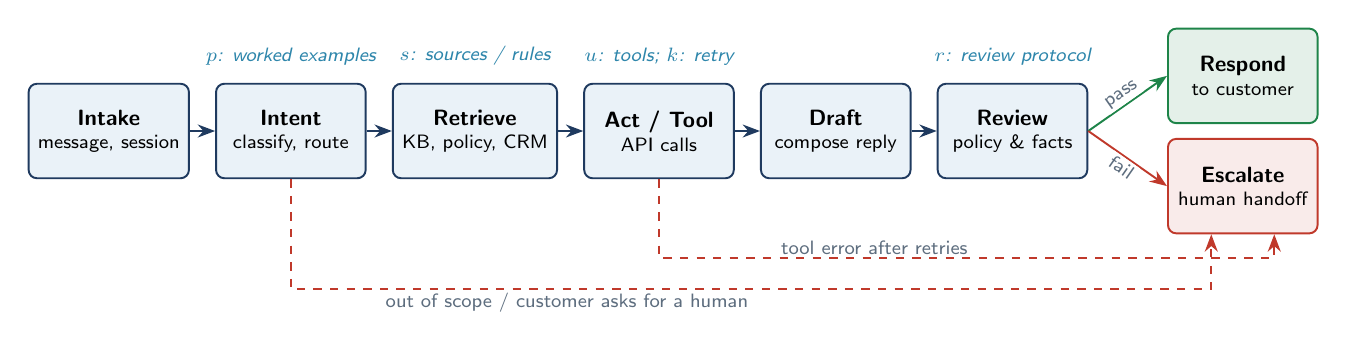
\begin{tikzpicture}[
  node distance=5mm and 3.2mm,
  box/.style={draw=navy, fill=soft, rounded corners=3pt, line width=0.7pt,
               minimum width=19mm, minimum height=12mm, align=center, font=\footnotesize},
  term/.style={box, fill=ok!12, draw=ok},
  esc/.style={box, fill=warn!10, draw=warn},
  theta/.style={font=\scriptsize\itshape, text=accent, align=center},
  arr/.style={-{Stealth[length=2.2mm]}, line width=0.7pt, draw=navy},
  lbl/.style={font=\scriptsize, text=muted, fill=white, inner sep=1pt}
]
\node[box] (intake)   {\textbf{Intake}\\[-1pt]\scriptsize message, session};
\node[box, right=of intake] (intent)   {\textbf{Intent}\\[-1pt]\scriptsize classify, route};
\node[box, right=of intent] (retrieve) {\textbf{Retrieve}\\[-1pt]\scriptsize KB, policy, CRM};
\node[box, right=of retrieve] (act)    {\textbf{Act / Tool}\\[-1pt]\scriptsize API calls};
\node[box, right=of act] (draft)       {\textbf{Draft}\\[-1pt]\scriptsize compose reply};
\node[box, right=of draft] (review)    {\textbf{Review}\\[-1pt]\scriptsize policy \& facts};
\node[term, right=10mm of review, yshift=7mm] (respond) {\textbf{Respond}\\[-1pt]\scriptsize to customer};
\node[esc,  right=10mm of review, yshift=-7mm] (escalate) {\textbf{Escalate}\\[-1pt]\scriptsize human handoff};

\draw[arr] (intake) -- (intent);
\draw[arr] (intent) -- (retrieve);
\draw[arr] (retrieve) -- (act);
\draw[arr] (act) -- (draft);
\draw[arr] (draft) -- (review);
\draw[arr, draw=ok] (review.east) -- node[lbl, above, sloped]{pass} (respond.west);
\draw[arr, draw=warn] (review.east) -- node[lbl, below, sloped]{fail} (escalate.west);
% early exits to escalation
\coordinate (laneA) at ($(escalate.south)+(0,-7mm)$);
\coordinate (laneB) at ($(escalate.south)+(0,-3mm)$);
\draw[arr, draw=warn, dashed] (intent.south) -- (intent.south |- laneA)
  -- node[lbl, pos=0.3, below]{out of scope / customer asks for a human} ($(laneA)+(-4mm,0)$) -- ($(escalate.south)+(-4mm,0)$);
\draw[arr, draw=warn, dashed] (act.south) -- (act.south |- laneB)
  -- node[lbl, pos=0.35, above]{tool error after retries} ($(laneB)+(4mm,0)$) -- ($(escalate.south)+(4mm,0)$);

% theta annotations
\node[theta, above=1mm of intent]   {$p$: worked examples};
\node[theta, above=1mm of retrieve] {$s$: sources / rules};
\node[theta, above=1mm of act]      {$u$: tools; $k$: retry};
\node[theta, above=1mm of review]   {$r$: review protocol};
\end{tikzpicture}
\end{center}
\vspace{-8pt}
{\scriptsize\color{muted} Typical CSR pipeline. Blue labels show which education component $\theta=(s,p,u,r,k)$ applies at each node.
Retries are bounded, so we unroll them into fixed copies of the node and the graph stays acyclic.\par}

\vspace{3pt}
\begin{minipage}[t]{0.49\linewidth}
\textbf{\color{navy}Why DAGs instead of free-form autonomous loops}
\begin{itemize}
  \item \textbf{Deterministic control flow:} the same inputs follow the same path, with no unbounded ``think--act'' loops.
  \item \textbf{Testability per node:} each node has its own input/output contract and its own eval set.
  \item \textbf{Easy auditing:} every turn produces a trace of the nodes visited, data retrieved, and tools called.
  \item \textbf{Safe retries:} retries are scoped to one node and capped; side-effecting tools use idempotency keys.
  \item \textbf{Clear escalation paths:} handoff is an explicit edge, not something the model has to decide to do.
\end{itemize}
\end{minipage}\hfill
\begin{minipage}[t]{0.48\linewidth}
\textbf{\color{navy}Comparison}\\[2pt]
\footnotesize
\begin{tabularx}{\linewidth}{@{}>{\raggedright\arraybackslash}p{19mm}XX@{}}
\toprule
 & \textbf{DAG agent} & \textbf{Autonomous loop} \\
\midrule
Control flow & Fixed, reviewable & Model decides each step \\
Testing      & Unit eval per node & End-to-end only \\
Audit trail  & Node-level trace & Long free-form transcript \\
Failure mode & Local, bounded & Can compound or loop \\
Cost/latency & Predictable & Varies widely \\
Escalation   & Explicit edge & Depends on the model \\
\bottomrule
\end{tabularx}
\end{minipage}

% ---------- Reliability framing ----------
\section{Reliability framing: reliability as an education optimization problem}
\begin{minipage}[t]{0.49\linewidth}\raggedright
This framing comes from our research repo
(\texttt{README.md}, \texttt{designing\_ai\_reliability\_as\_an\_\allowbreak education\_optimization\_problem.md}).
We treat the foundation model as a \textbf{fixed student}: we do not change its weights. Instead we
optimize the \textbf{education vector} $\theta=(s,p,u,r,k)$ that we give it:
\[
\theta^\star=\arg\max_{\theta}\; \mathrm{LB}(\theta)-\lambda\,\hat V(\theta)
\]
subject to a cost budget and \textbf{zero policy violations}. Here LB is the Wilson lower bound on the
strict-pass rate on unseen tasks, and $\hat V$ is the variance across runs. The DAG is what makes this
practical: each component of $\theta$ maps to a specific node that we can change and measure on its own.
\end{minipage}\hfill
\begin{minipage}[t]{0.48\linewidth}
\footnotesize
\begin{tabularx}{\linewidth}[t]{@{}>{\bfseries}l>{\raggedright\arraybackslash}X@{}}
\toprule
$\theta$ & \textbf{Meaning $\rightarrow$ CSR equivalent} \\
\midrule
$s$ Sources  & Reference rules / handbook $\rightarrow$ policy KB, refund rules \\
$p$ Practice & Worked examples $\rightarrow$ few-shot resolved tickets \\
$u$ Tools    & Executable checks, retrieval $\rightarrow$ CRM, order and booking APIs \\
$r$ Review   & Self-check before submitting $\rightarrow$ policy/compliance node \\
$k$ Retry    & Retakes on feedback $\rightarrow$ bounded node retries \\
\bottomrule
\end{tabularx}

\vspace{3pt}
\textbf{What the research shows so far:} most failures are \emph{compliance} failures (breaking a rule)
rather than \emph{capability} failures. Explicit sources ($s$) and an automated policy-check
retry ($k$) fix most of them cheaply; in the paper's factorial study, retries rescued 17 of 17
compliance failures. For CSR agents this means investing first in the Retrieve, Review, and retry
parts of the graph.
\end{minipage}

\vfill
{\color{accent}\rule{\linewidth}{0.4pt}}\\[-1pt]
{\scriptsize\color{muted} Source: \texttt{docs/csr\_dag\_agent\_onepager.tex} in
\href{https://github.com/cosmosanalytics/AI-reliability-as-education-optimization}{cosmosanalytics/AI-reliability-as-education-optimization}.
See the full manuscript for the formalism, the experimental design, and its limitations.}
\end{document}
